% Research-paper source. Compile from paper/: tectonic --outdir drafts track2.tex
% Options for packages loaded elsewhere
\PassOptionsToPackage{unicode}{hyperref}
\PassOptionsToPackage{hyphens}{url}
\documentclass[
  10pt,
]{article}
\usepackage{xcolor}
\usepackage[a4paper,margin=0.65in]{geometry}
\usepackage{amsmath,amssymb}
\setcounter{secnumdepth}{-\maxdimen} % remove section numbering
\usepackage{iftex}
\ifPDFTeX
  \usepackage[T1]{fontenc}
  \usepackage[utf8]{inputenc}
  \usepackage{textcomp} % provide euro and other symbols
\else % if luatex or xetex
  \usepackage{unicode-math} % this also loads fontspec
  \defaultfontfeatures{Scale=MatchLowercase}
  \defaultfontfeatures[\rmfamily]{Ligatures=TeX,Scale=1}
\fi
\usepackage{lmodern}
\ifPDFTeX\else
  % xetex/luatex font selection
\fi
% Use upquote if available, for straight quotes in verbatim environments
\IfFileExists{upquote.sty}{\usepackage{upquote}}{}
\IfFileExists{microtype.sty}{% use microtype if available
  \usepackage[]{microtype}
  \UseMicrotypeSet[protrusion]{basicmath} % disable protrusion for tt fonts
}{}
\makeatletter
\@ifundefined{KOMAClassName}{% if non-KOMA class
  \IfFileExists{parskip.sty}{%
    \usepackage{parskip}
  }{% else
    \setlength{\parindent}{0pt}
    \setlength{\parskip}{6pt plus 2pt minus 1pt}}
}{% if KOMA class
  \KOMAoptions{parskip=half}}
\makeatother
\usepackage{longtable,booktabs,array}
\usepackage{caption}
\captionsetup[table]{skip=6pt}
\newcounter{none} % for unnumbered tables
\usepackage{calc} % for calculating minipage widths
% Correct order of tables after \paragraph or \subparagraph
\usepackage{etoolbox}
\makeatletter
\patchcmd\longtable{\par}{\if@noskipsec\mbox{}\fi\par}{}{}
\makeatother
\usepackage{graphicx}
\makeatletter
\newsavebox\pandoc@box
\newcommand*\pandocbounded[1]{% scales image to fit in text height/width
  \sbox\pandoc@box{#1}%
  \Gscale@div\@tempa{\textheight}{\dimexpr\ht\pandoc@box+\dp\pandoc@box\relax}%
  \Gscale@div\@tempb{\linewidth}{\wd\pandoc@box}%
  \ifdim\@tempb\p@<\@tempa\p@\let\@tempa\@tempb\fi% select the smaller of both
  \ifdim\@tempa\p@<\p@\scalebox{\@tempa}{\usebox\pandoc@box}%
  \else\usebox{\pandoc@box}%
  \fi%
}
% Set default figure placement to htbp
\def\fps@figure{htbp}
\makeatother
\setlength{\emergencystretch}{3em} % prevent overfull lines
\providecommand{\tightlist}{%
  \setlength{\itemsep}{0pt}\setlength{\parskip}{0pt}}
\usepackage{bookmark}
\IfFileExists{xurl.sty}{\usepackage{xurl}}{} % add URL line breaks if available
\urlstyle{same}
% fallback for those not using the hyperref driver hyperxmp:
\makeatletter
\@ifundefined{xmpquote}{\newcommand{\xmpquote}[1]{#1}}{}
\makeatother
\hypersetup{
  hidelinks,
  pdfcreator={LaTeX via pandoc}}

\author{}
\date{}


\usepackage{microtype}
\usepackage{etoolbox}
\AtBeginEnvironment{longtable}{\small}
\setlength{\parindent}{1em}
\setlength{\parskip}{3pt}
\AtBeginDocument{\fontsize{10.5}{12}\selectfont}
\emergencystretch=2em

\begin{document}
\begin{center}
{\LARGE\bfseries Extreme events: a shift or a change in shape?\par}
\vspace{6pt}
{\small Environmental Economics -- BSc AIDAMS -- Track 2\par}
\end{center}


\section*{Abstract}\label{abstract}

We compare heat and drought distributions in Spain, France, Germany and
Sweden using country-level ERA5-Land indices. Fixed historical
thresholds, mean-shift benchmarks and quantile regressions distinguish
changes in overall levels from additional tail movement. Heat-threshold
crossings increase across countries; a shift in the mean accounts for
much of the rise. France and Germany also show wider pooled temperature
distributions, while evidence of extra upper-tail movement remains
imprecise. Drought results vary more across countries and thresholds.
The estimates describe historical changes; small tail samples and
limitations of the early reanalysis record constrain inference.

\section{1. Question}\label{question}

Have heat and drought extremes become more frequent or more intense in
Spain, France, Germany and Sweden, and how much of that change can be
described by a shift in the mean? We compare 1961-1990 with 1996-2025
using country-level ERA5-Land data from the Copernicus Interactive
Climate Atlas. Our central question is whether the recent distribution
resembles the early distribution moved to a new level, or whether its
extreme tail has moved further than the mean.

The distinction matters for risk assessment. A fixed historical
threshold can be crossed much more often after the mean changes, even if
variability around the mean stays constant. More exceedances therefore
do not, by themselves, establish that a tail has become heavier. For
water managers, agricultural producers and planners, both the level of
the climate variable and the distribution around that level matter. Our
data measure climate conditions; they do not measure economic losses or
identify the benefits of an adaptation policy.

Three references frame the question. IPCC AR6 Chapter 11 documents
changes in the frequency and intensity of temperature extremes and
assesses their human contribution using evidence beyond simple
historical comparisons (Seneviratne et al., 2021, Sections 11.2-11.3).
Hansen, Sato and Ruedy (2012) show a shift toward hotter seasonal
temperature anomalies and a larger occurrence of exceptionally hot
summers. Rhines and Huybers (2013) question the inference of increased
variability from those distributions: normalisation, trends and changing
station coverage can produce apparent widening. Their result makes the
empirical task clear. We must compare tail changes with a shift
benchmark, rather than infer a change in shape from an increase in
extremes alone. These papers concern seasonal temperatures and different
spatial aggregations; our analysis is not a direct replication.

We use two complementary indices: monthly TXx for June-August, measuring
the country average of local monthly temperature maxima, and September
SPEI-6, summarising April-September climatic water balance. The four
countries span southern to northern Europe, allowing us to compare
contrasting climates within one dataset. TXx values are expressed
relative to each country\textquotesingle s early-period mean for the
same calendar month. We examine its upper tail at P75, P90, P95 and P99.
For SPEI-6, lower values mean drier conditions, so the corresponding
thresholds are P25, P10, P5 and P1.

An answer requires three comparisons: the change in the mean and spread;
the change in tail percentiles relative to the mean; and the frequency
of crossing fixed early-period thresholds. Time trends and quantile
regressions provide a further check on whether the centre and tails move
at different rates. The results describe these four country-level series
over the observed record. They do not attribute individual events to
greenhouse gas emissions or predict future extremes.

\clearpage

\section{2. Data}\label{data}

Our data come from the Copernicus Interactive Climate Atlas
(\url{https://atlas.climate.copernicus.eu/}, version v2.5), produced by the
Copernicus Climate Change Service (C3S). The Atlas is built on the
gridded dataset that C3S publishes on the Climate Data Store (C3S,
2024b). We downloaded the series through the Atlas\textquotesingle s
regional-information export on 29 October 2026. All series come from
ERA5-Land, a land-surface reanalysis that ECMWF produces for C3S by
re-running the land component of the ERA5 model on a 0.1° regular grid;
the Atlas retains this native resolution (C3S, 2023). We study four
European countries along a south-north gradient: Spain, France, Germany
and Sweden. Every series is annual and covers 1950 to 2025, giving 76
observations per series. A validation script (scripts/check\_raw.py)
confirms that all 16 files share the same Atlas version and dataset,
that each year from 1950 to 2025 appears exactly once, and that no
observation is missing. We therefore carry out no imputation or
interpolation. The label "1961-1990" in the file headers refers to the
period the Atlas highlights in its charts; it does not restrict the
data.

We use two indices. The first, TXx, is the monthly maximum of daily
maximum near-surface air temperature, in degrees Celsius. In each grid
cell, the daily maximum is the highest of the hourly 2 m temperatures of
that day, and the Atlas takes the highest of these daily maxima in a
given month (C3S, 2023). It then averages these cell values over the
country\textquotesingle s territory, weighting each cell of the regular
latitude-longitude grid by the cosine of its latitude; since ERA5-Land
covers land only, sea cells do not enter the average (C3S, 2024a). Our
country-level TXx is therefore the average across the country of each
location\textquotesingle s hottest day of the month, not the single
hottest value recorded anywhere in the country. We use TXx for June,
July and August. Pooling the three summer months gives 90 observations
per 30-year period instead of the 30 that a single month would provide.
This matters because our question concerns the tails of the
distribution, which are poorly estimated in small samples. The cost is
that the three months are not independent draws from one distribution,
as August is typically hotter than June. Any pooled comparison must
allow for this seasonal difference.

The second index is the Standardised Precipitation-Evapotranspiration
Index over a six-month window (SPEI-6). For each grid cell, the balance
between precipitation and potential evapotranspiration (PET) is
accumulated over the preceding six months. It is then transformed, by
fitting a probability distribution, into standard deviations from the
mean of a reference period of 1971-2005. The Atlas documentation is
inconsistent on this point: the dataset documentation gives 1971-2010
(C3S, 2023), while the v2.5 changelog gives 1971-2005 in the context of
projections (C3S, 2024a). The Atlas information panel for SPEI-6,
however, states explicitly that the reference period is 1971-2005 "for
observations, reanalysis, and projections" (verbatim copy in
data/atlas\_info\_spei6.txt), and we report this value. Potential
evapotranspiration is computed with the Hargreaves formulation
(Hargreaves and Samani, 1985), which the Atlas has used since version
2.0 (C3S, 2024a), implemented with the xclim library (C3S, 2023). The
index has no units; negative values indicate conditions drier than the
reference climate and positive values wetter ones. As with TXx, the
Atlas averages the grid-cell values over each country. We keep only the
September value in each year. Because the window is six months long, the
September value summarises the water balance from April to September,
that is, the whole growing and warm season. Taking one month per year
also avoids the strong autocorrelation that consecutive monthly SPEI-6
values would introduce, as they share five of their six months. Each
year then contributes one non-overlapping observation of warm-season
dryness.

\clearpage

\subsection{Data limitations}\label{data-limitations}

These data have several limitations. First, ERA5-Land is a reanalysis,
not a set of station observations. It combines a numerical model with
assimilated observations, and its representation of extremes depends on
the model\textquotesingle s physics as well as on the observations. A
specific concern affects the start of our sample: the Atlas disables
ERA5-Land trends before 1978 because of a potential inconsistency in the
ERA5 forcing used for that period (C3S, 2024a). Our early period
overlaps these years, so part of any difference between the early and
recent distributions could be a data artefact rather than a change in
climate.

Second, averaging over a country smooths local extremes. A heatwave or
drought that affects only part of the territory is diluted in the
national mean, so our series understate the severity of the most extreme
local events, and the smoothing is likely to be stronger for large or
climatically diverse countries such as France and Spain. In addition,
the Atlas documentation does not state how grid cells that straddle a
national border are treated (C3S, 2024a), so the exact spatial footprint
of each country average is not known.

Third, SPEI depends on modelling choices: the reference period sets the
zero of the scale, and the PET formulation determines how strongly
rising temperatures translate into apparent drying. A different
reference period or PET method could shift the series or change their
trends.

Fourth, standardisation is done per grid cell, and averaging
standardised values across cells reduces their variance. The
country-level SPEI-6 series have standard deviations between 0.754 and
0.902, all below the unit variance of a cell-level index, and their
1950-2025 means are negative, between -0.285 and -0.037. As a result,
the Atlas\textquotesingle s fixed threshold of -1.5 for "severe" drought
is rarely crossed at the country level, and a count of exceedances of
that threshold would carry little information. We therefore define
extremes with percentile thresholds taken from each
country\textquotesingle s own distribution.

Finally, the tails contain few observations by construction. With 76
years per series, or 90 observations per 30-year period for pooled TXx,
the 90th or 95th percentile within a period is estimated from only a
handful of values. Estimates of tail shape are thus imprecise. Section 5
reports bootstrap intervals that keep the three months of a summer
together when resampling; these do not account for dependence across
years.

\clearpage

\section{3. Summary statistics}\label{summary-statistics}

We compare 1961-1990 (early, E) with 1996-2025 (recent, R). TXx pools
June-August anomalies relative to the early mean of the same country and
month. SPEI-6 is used as published, one September value per year. The
distributions contain 90 TXx values or 30 SPEI-6 values per country and
period. Percentiles use linear interpolation.

Table 1. Summary statistics: early and recent distributions.

{\def\LTcaptype{none} % do not increment counter
\begin{longtable}[]{@{}
  >{\centering\arraybackslash}p{(\linewidth - 18\tabcolsep) * \real{0.1019}}
  >{\centering\arraybackslash}p{(\linewidth - 18\tabcolsep) * \real{0.1091}}
  >{\centering\arraybackslash}p{(\linewidth - 18\tabcolsep) * \real{0.0986}}
  >{\centering\arraybackslash}p{(\linewidth - 18\tabcolsep) * \real{0.0986}}
  >{\centering\arraybackslash}p{(\linewidth - 18\tabcolsep) * \real{0.0986}}
  >{\centering\arraybackslash}p{(\linewidth - 18\tabcolsep) * \real{0.0986}}
  >{\centering\arraybackslash}p{(\linewidth - 18\tabcolsep) * \real{0.0986}}
  >{\centering\arraybackslash}p{(\linewidth - 18\tabcolsep) * \real{0.0986}}
  >{\centering\arraybackslash}p{(\linewidth - 18\tabcolsep) * \real{0.0986}}
  >{\centering\arraybackslash}p{(\linewidth - 18\tabcolsep) * \real{0.0986}}@{}}
\toprule\noalign{}
\begin{minipage}[b]{\linewidth}\centering
\textbf{Index}
\end{minipage} & \begin{minipage}[b]{\linewidth}\centering
\textbf{Country}
\end{minipage} & \begin{minipage}[b]{\linewidth}\centering
\textbf{Period}
\end{minipage} & \begin{minipage}[b]{\linewidth}\centering
\textbf{N}
\end{minipage} & \begin{minipage}[b]{\linewidth}\centering
\textbf{Mean}
\end{minipage} & \begin{minipage}[b]{\linewidth}\centering
\textbf{SD}
\end{minipage} & \begin{minipage}[b]{\linewidth}\centering
\textbf{Min}
\end{minipage} & \begin{minipage}[b]{\linewidth}\centering
\textbf{P5}
\end{minipage} & \begin{minipage}[b]{\linewidth}\centering
\textbf{P95}
\end{minipage} & \begin{minipage}[b]{\linewidth}\centering
\textbf{Max}
\end{minipage} \\
\midrule\noalign{}
\endhead
\bottomrule\noalign{}
\endlastfoot
TXx & ESP & E & 90 & 0.00 & 1.61 & -5.05 & -2.86 & 2.03 & 4.06 \\
TXx & ESP & R & 90 & 2.10 & 1.74 & -2.16 & -0.69 & 5.31 & 5.89 \\
TXx & FRA & E & 90 & 0.00 & 1.83 & -3.57 & -2.73 & 3.16 & 4.27 \\
TXx & FRA & R & 90 & 2.44 & 2.35 & -4.04 & -1.02 & 6.35 & 8.21 \\
TXx & GER & E & 90 & 0.00 & 1.78 & -4.63 & -2.95 & 2.89 & 4.01 \\
TXx & GER & R & 90 & 1.85 & 2.37 & -4.12 & -1.91 & 5.29 & 6.74 \\
TXx & SWE & E & 90 & 0.00 & 2.06 & -4.85 & -3.76 & 3.18 & 4.61 \\
TXx & SWE & R & 90 & 0.63 & 2.15 & -4.45 & -2.76 & 4.18 & 4.98 \\
SPEI-6 & ESP & E & 30 & 0.15 & 0.75 & -1.02 & -0.89 & 1.44 & 2.30 \\
SPEI-6 & ESP & R & 30 & -0.62 & 0.70 & -1.82 & -1.63 & 0.59 & 0.80 \\
SPEI-6 & FRA & E & 30 & 0.05 & 0.86 & -1.70 & -1.40 & 1.15 & 1.25 \\
SPEI-6 & FRA & R & 30 & -0.56 & 0.77 & -1.98 & -1.56 & 0.41 & 0.85 \\
SPEI-6 & GER & E & 30 & 0.21 & 0.82 & -1.90 & -1.04 & 1.31 & 1.70 \\
SPEI-6 & GER & R & 30 & -0.36 & 0.91 & -2.80 & -1.95 & 0.82 & 0.97 \\
SPEI-6 & SWE & E & 30 & -0.10 & 0.68 & -1.99 & -1.27 & 0.99 & 1.26 \\
SPEI-6 & SWE & R & 30 & 0.07 & 0.80 & -1.89 & -1.15 & 1.42 & 1.56 \\
\end{longtable}
}

TXx: anomalies in °C. SPEI-6: dimensionless, negative = drier. E:
1961-1990; R: 1996-2025. Country codes: Spain (ESP), France (FRA),
Germany (GER), Sweden (SWE). Source: C3S Atlas v2.5, ERA5-Land, accessed
29 October 2026; our calculations. Full quantiles:
outputs/summary\_stats.csv.

\textbf{Table 2. TXx reference levels: 1961-1990 mean, °C.}

{\def\LTcaptype{none} % do not increment counter
\begin{longtable}[]{@{}
  >{\centering\arraybackslash}p{(\linewidth - 6\tabcolsep) * \real{0.2500}}
  >{\centering\arraybackslash}p{(\linewidth - 6\tabcolsep) * \real{0.2500}}
  >{\centering\arraybackslash}p{(\linewidth - 6\tabcolsep) * \real{0.2500}}
  >{\centering\arraybackslash}p{(\linewidth - 6\tabcolsep) * \real{0.2500}}@{}}
\toprule\noalign{}
\begin{minipage}[b]{\linewidth}\centering
\textbf{Country}
\end{minipage} & \begin{minipage}[b]{\linewidth}\centering
\textbf{June}
\end{minipage} & \begin{minipage}[b]{\linewidth}\centering
\textbf{July}
\end{minipage} & \begin{minipage}[b]{\linewidth}\centering
\textbf{August}
\end{minipage} \\
\midrule\noalign{}
\endhead
\bottomrule\noalign{}
\endlastfoot
ESP & 30.14 & 33.31 & 32.90 \\
FRA & 26.85 & 29.59 & 28.97 \\
GER & 26.86 & 28.29 & 28.19 \\
SWE & 23.27 & 24.06 & 22.27 \\
\end{longtable}
}

TXx is higher in the recent period in all four countries. Mean shifts
are larger in Spain, France and Germany than in Sweden. The P95 rises
more than the mean in each country; Section 5 assesses the precision of
that extra movement. France and Germany also show wider pooled
distributions. SPEI-6 shifts toward drier conditions in Spain, France
and Germany, while Sweden changes little. Tail precision is limited:
each period has only five TXx observations above its own P95 and two
SPEI-6 observations below its own P5.

\clearpage

\section{4. Figures}\label{figures}

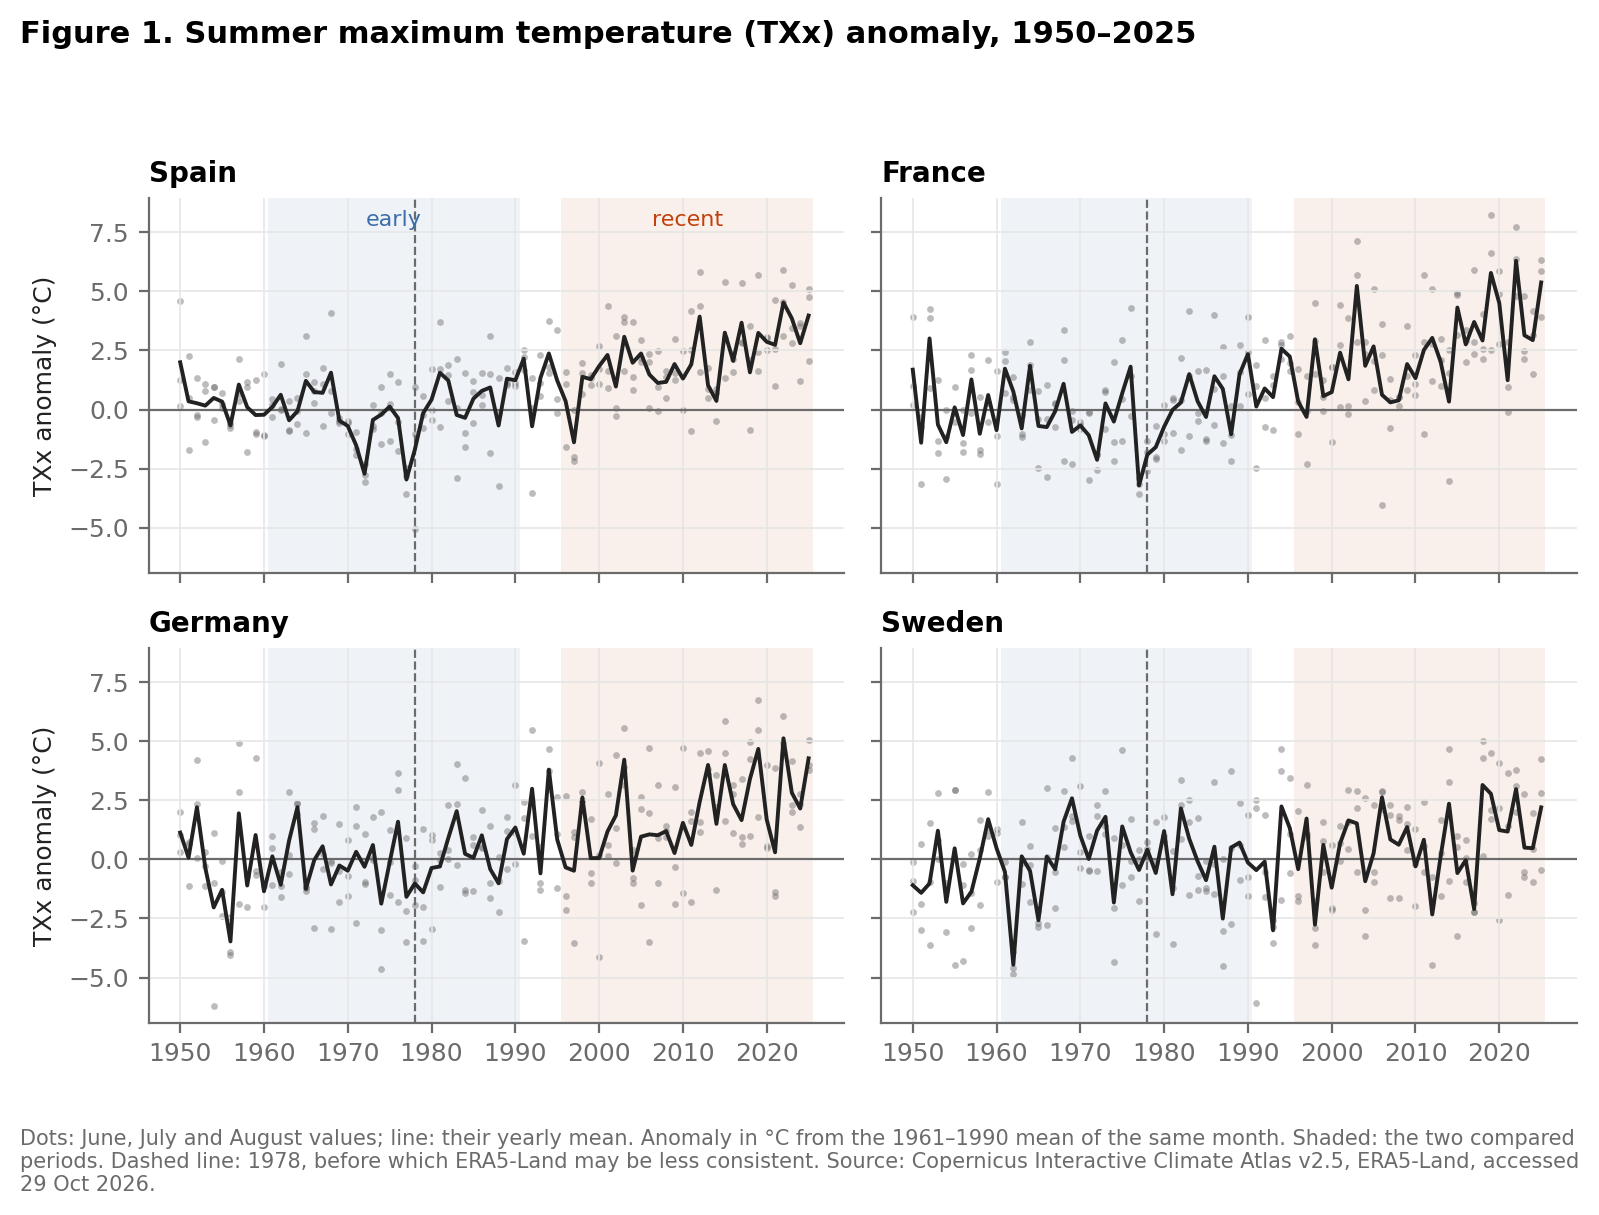
\includegraphics[width=5.65in,height=4.29315in]{../outputs/figures/fig1_txx_timeseries.png}

\textbf{Figure 1.} Country-average summer TXx anomalies show upward
trends with substantial year-to-year variation.

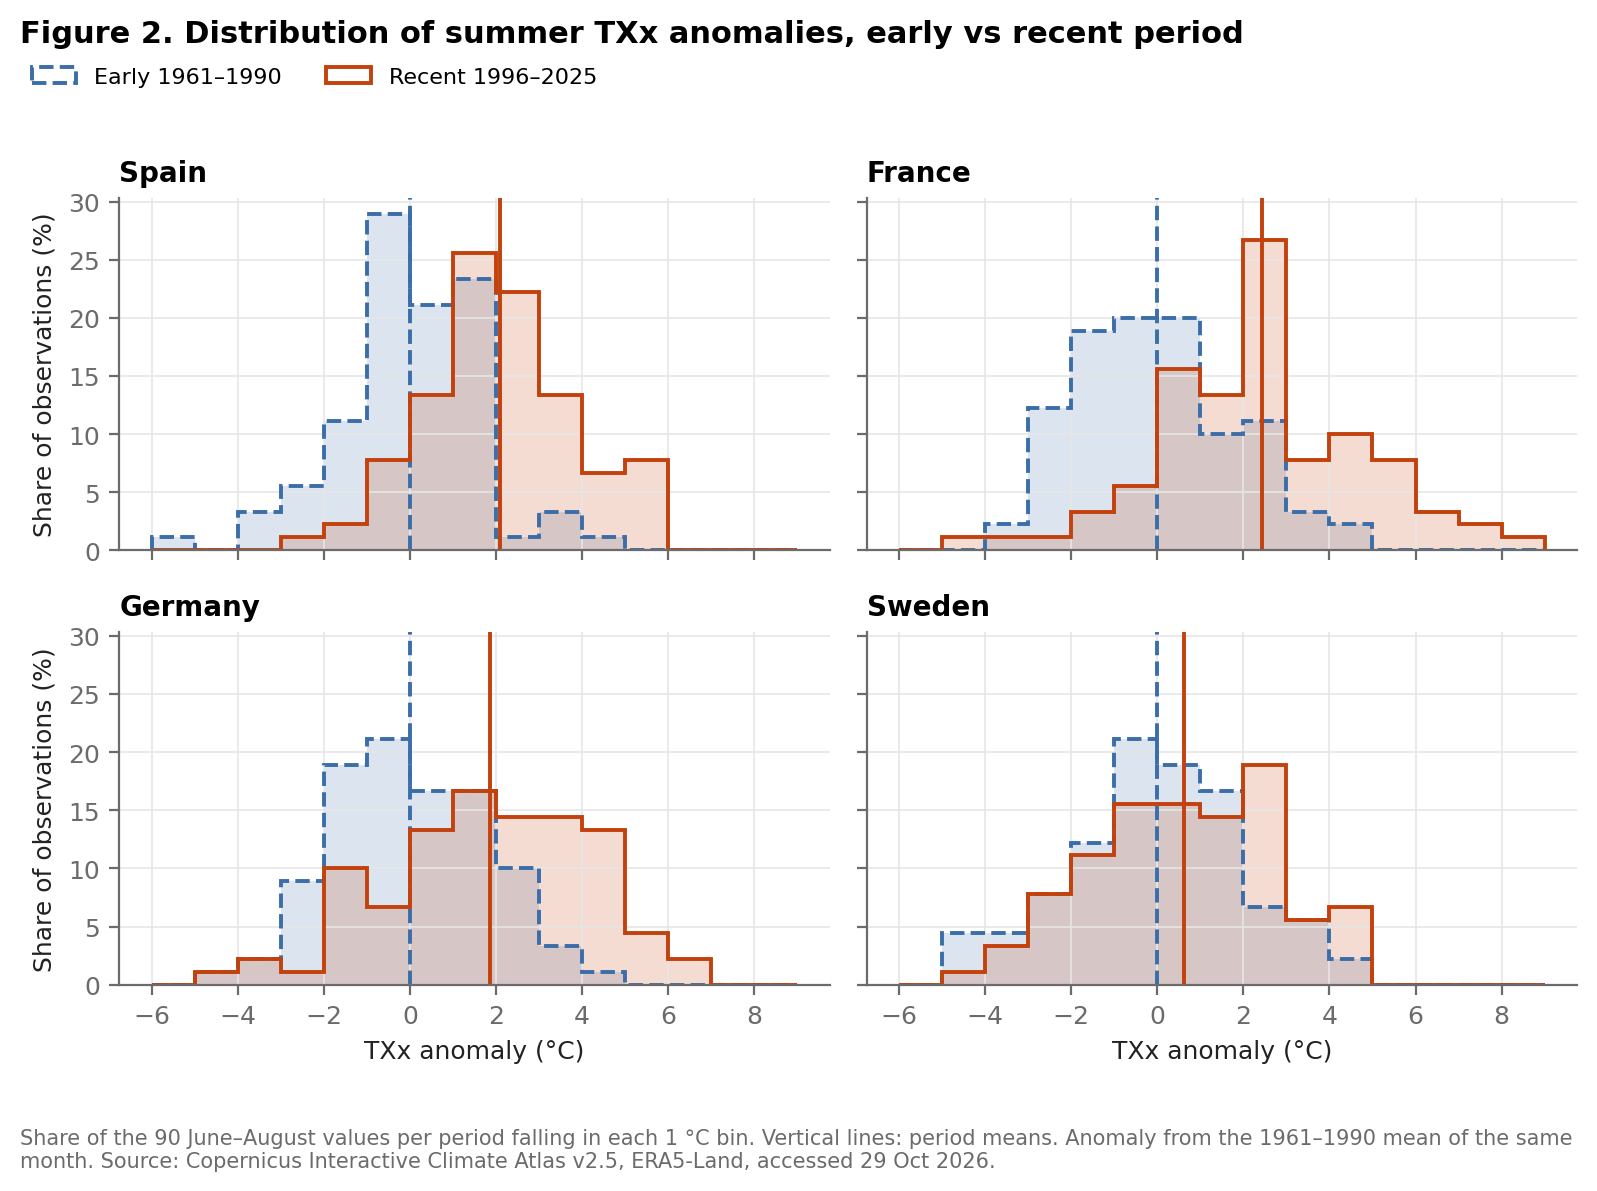
\includegraphics[width=5.65in,height=4.21362in]{../outputs/figures/fig2_txx_distributions.png}

\textbf{Figure 2.} Recent TXx distributions lie further toward hot
anomalies in Spain, France and Germany; Sweden\textquotesingle s
distributions overlap more.

\clearpage

\section{4. Figures}\label{figures-1}

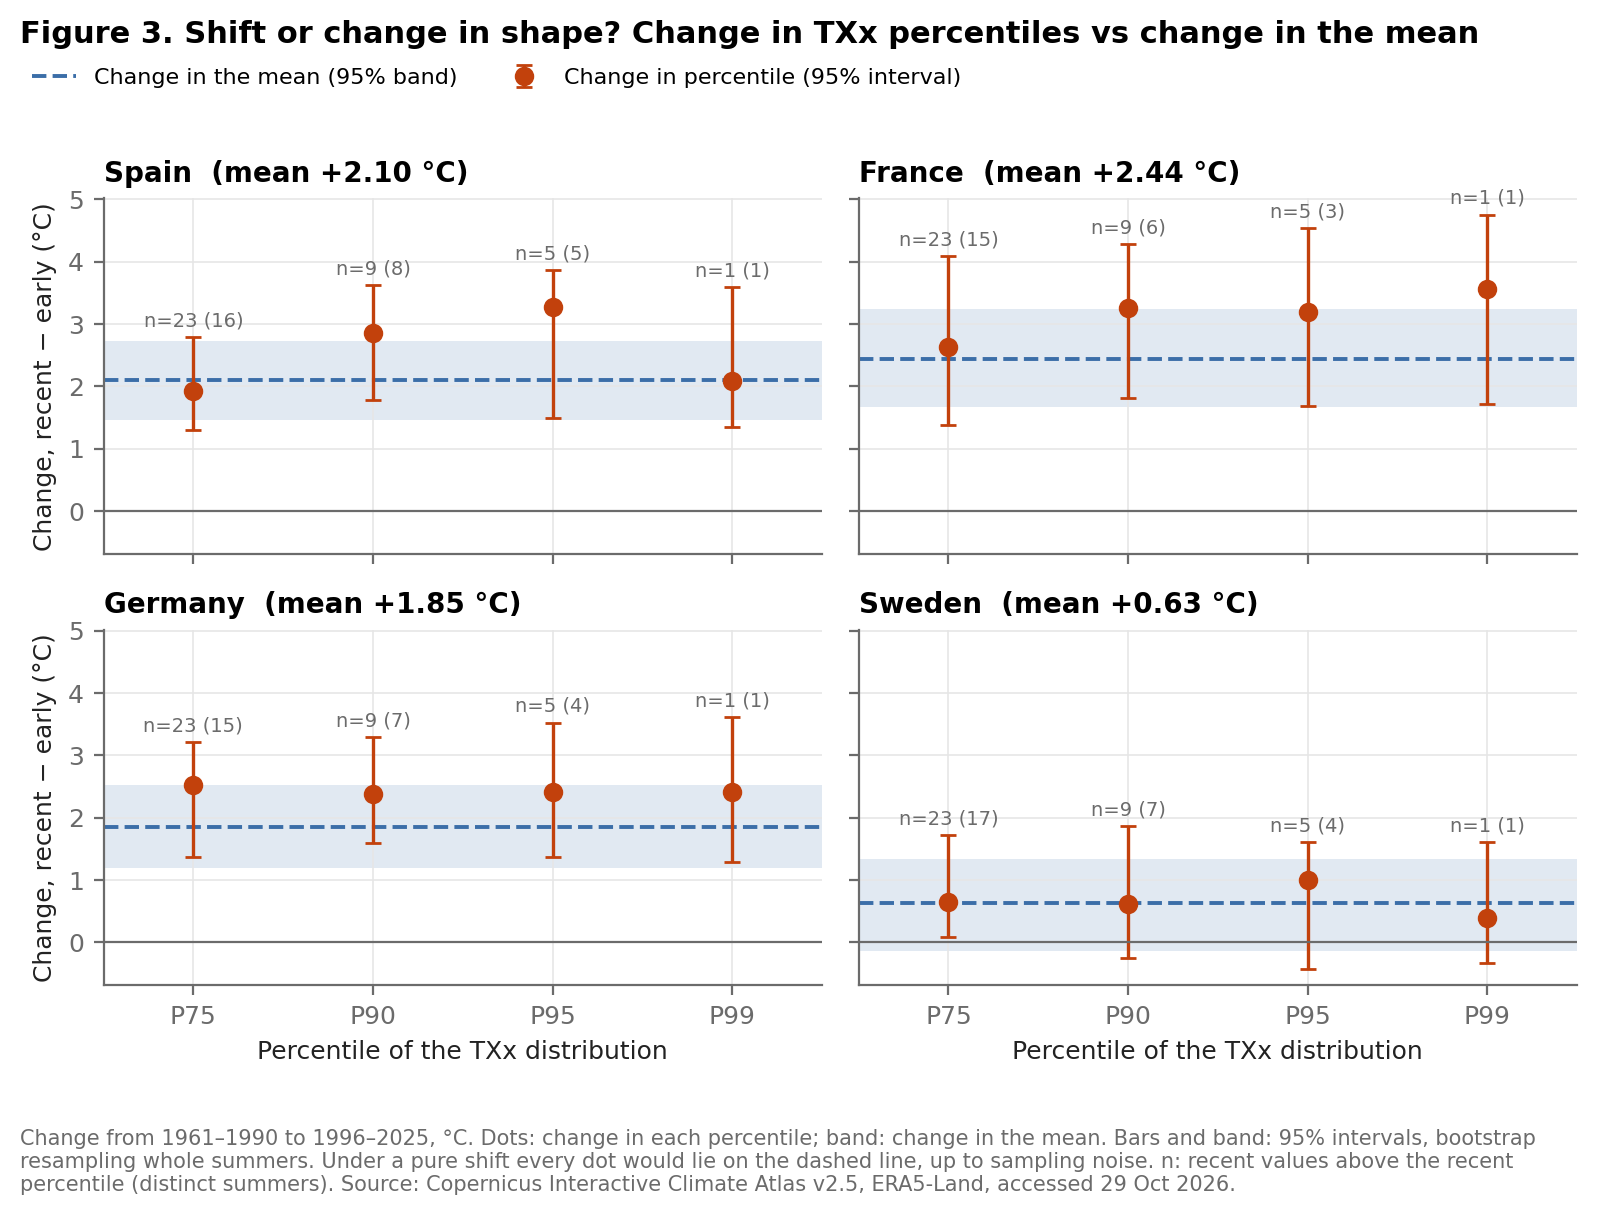
\includegraphics[width=5.65in,height=4.29853in]{../outputs/figures/fig3_txx_shift_vs_shape.png}

\textbf{Figure 3.} TXx upper percentiles rise, but their extra movement
relative to the mean is imprecise in every country.

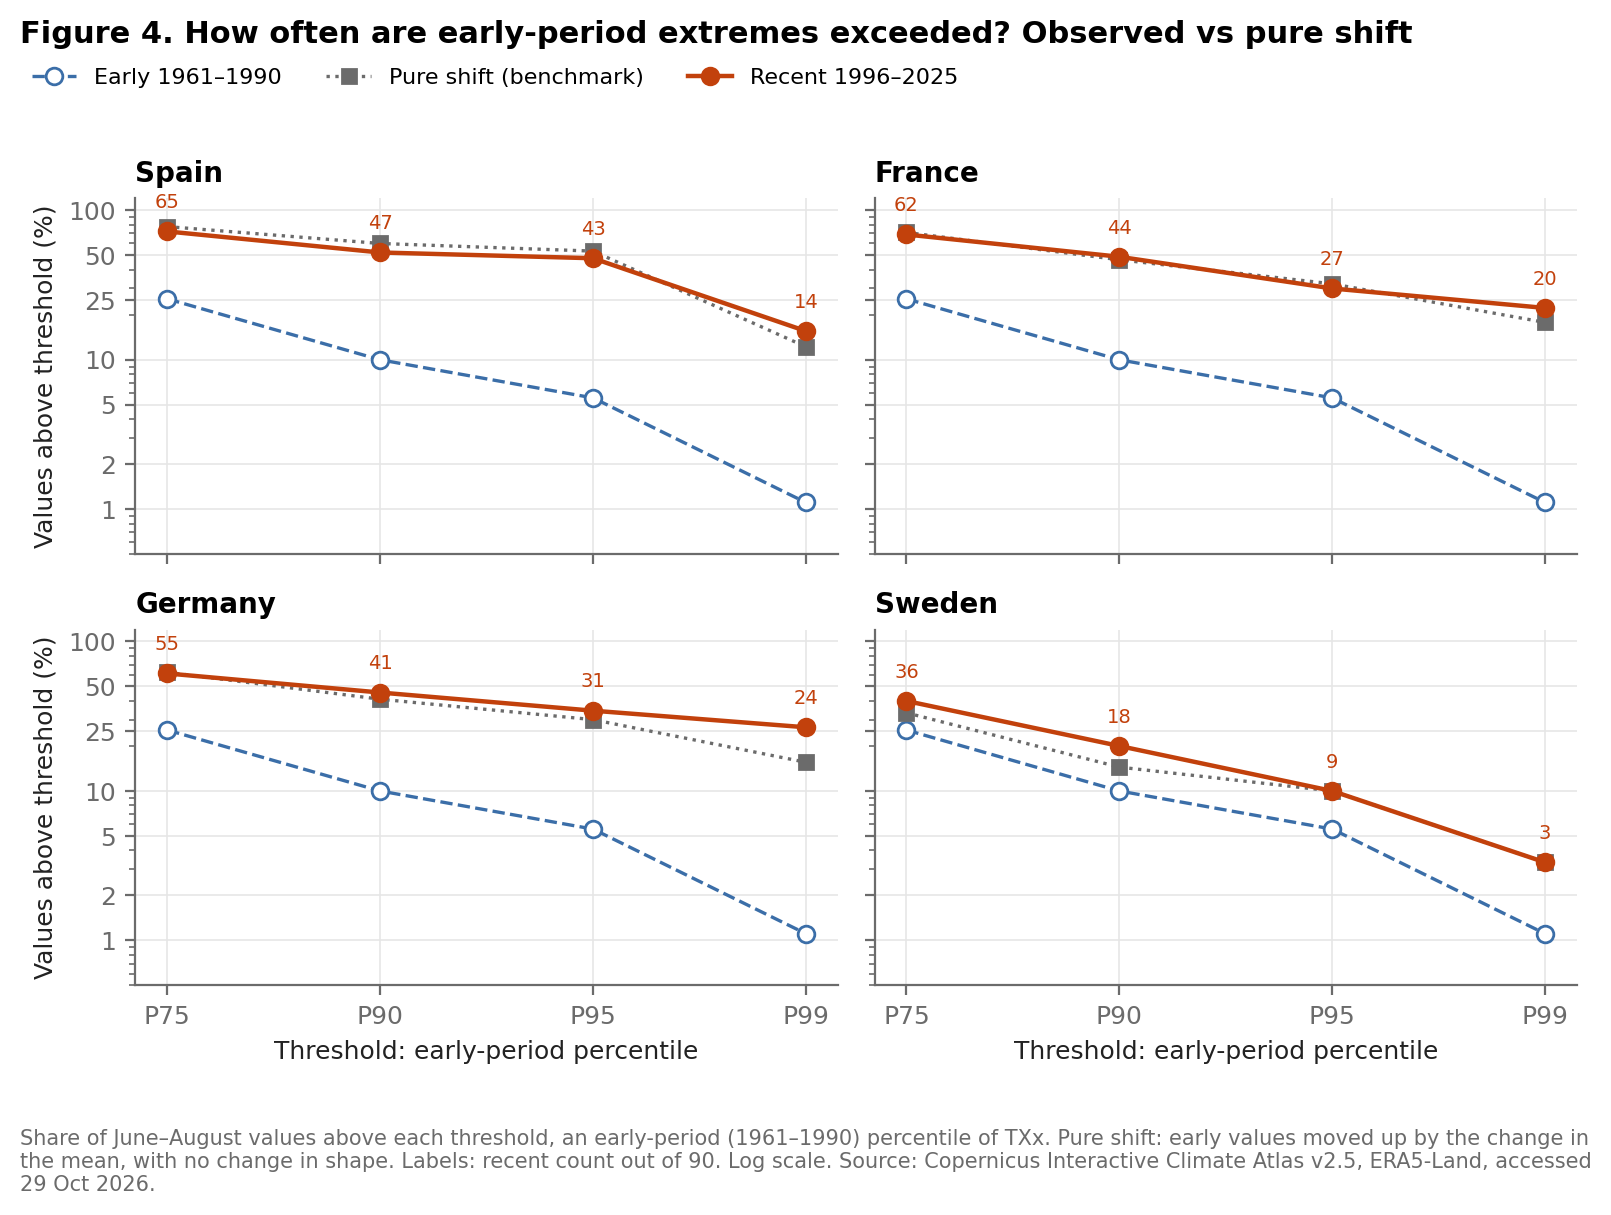
\includegraphics[width=5.65in,height=4.26117in]{../outputs/figures/fig4_txx_thresholds.png}

\textbf{Figure 4.} Heat exceedances increase at every threshold; the
shift benchmark accounts for much of the rise, with a larger gap at
Germany\textquotesingle s P99.

\clearpage

\section{4. Figures}\label{figures-2}

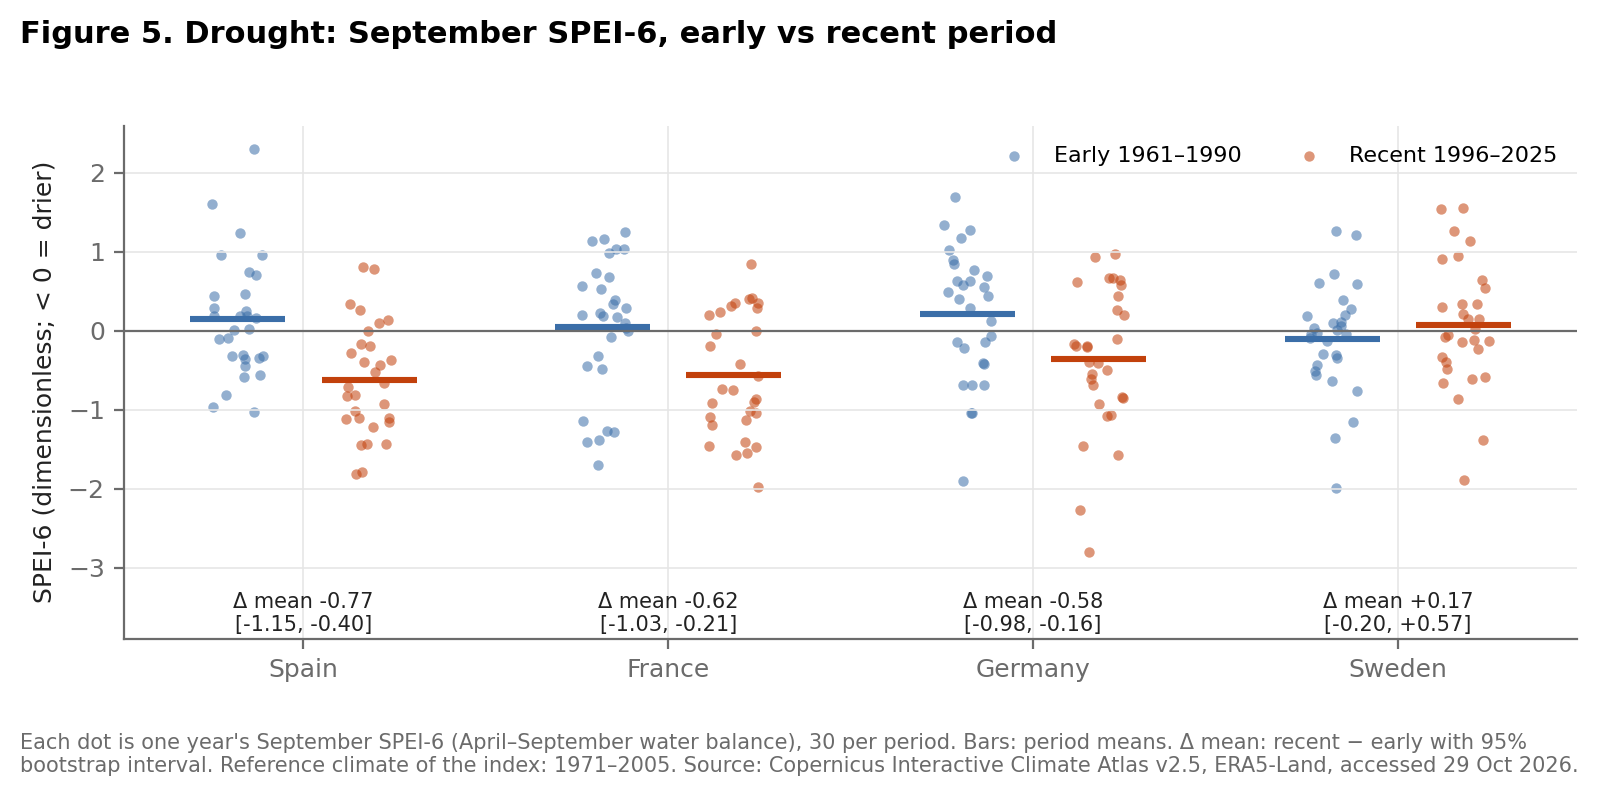
\includegraphics[width=6.7in,height=3.33742in]{../outputs/figures/fig5_spei_drought.png}

\textbf{Figure 5.} Mean September SPEI-6 falls in Spain, France and
Germany; Sweden shows no clear change between periods.

Each point represents one September value, covering April-September
climatic water balance; there are 30 observations per country and
period. Mean changes are -0.77 in Spain, -0.62 in France and -0.58 in
Germany, with 95\% intervals excluding zero, and +0.17 in Sweden, with
an interval including zero. Only two observations lie below each
period\textquotesingle s own P5. The estimates therefore provide limited
information about changes in the most severe drought tail.

The fixed-threshold comparison and the quantile regressions in Section 5
assess whether these changes extend beyond a shift in the mean. A
national index can change substantially without identifying a change in
local event duration or an economic loss.

\clearpage

\section{5. Econometrics}\label{econometrics}

\subsection{5.1. Fixed thresholds and a shift
benchmark}\label{fixed-thresholds-and-a-shift-benchmark}

We set each country\textquotesingle s thresholds on 1961-1990 and apply
the same values to 1996-2025. Frequency is the share of observations
above the TXx threshold or below the SPEI-6 threshold, not a count of
distinct heatwaves or drought episodes. Let the mean shift be

\[\Delta = {\bar{y}}_{R} - {\bar{y}}_{E}.\]

The shift benchmark adds delta to every early observation and recounts
exceedances. It preserves the early distribution\textquotesingle s shape
and uses the observed mean change; it is a descriptive benchmark, not an
independent forecast.

\textbf{Table 3. Threshold sensitivity: early count / recent count /
shift-benchmark count.}

{\def\LTcaptype{none} % do not increment counter
\begin{longtable}[]{@{}
  >{\centering\arraybackslash}p{(\linewidth - 10\tabcolsep) * \real{0.1019}}
  >{\centering\arraybackslash}p{(\linewidth - 10\tabcolsep) * \real{0.1092}}
  >{\centering\arraybackslash}p{(\linewidth - 10\tabcolsep) * \real{0.1972}}
  >{\centering\arraybackslash}p{(\linewidth - 10\tabcolsep) * \real{0.1972}}
  >{\centering\arraybackslash}p{(\linewidth - 10\tabcolsep) * \real{0.1972}}
  >{\centering\arraybackslash}p{(\linewidth - 10\tabcolsep) * \real{0.1972}}@{}}
\toprule\noalign{}
\begin{minipage}[b]{\linewidth}\centering
\textbf{Index}
\end{minipage} & \begin{minipage}[b]{\linewidth}\centering
\textbf{Country}
\end{minipage} & \begin{minipage}[b]{\linewidth}\centering
\textbf{P75 / P25}
\end{minipage} & \begin{minipage}[b]{\linewidth}\centering
\textbf{P90 / P10}
\end{minipage} & \begin{minipage}[b]{\linewidth}\centering
\textbf{P95 / P5}
\end{minipage} & \begin{minipage}[b]{\linewidth}\centering
\textbf{P99 / P1}
\end{minipage} \\
\midrule\noalign{}
\endhead
\bottomrule\noalign{}
\endlastfoot
TXx & Spain & 23 / 65 / 70 & 9 / 47 / 54 & 5 / 43 / 48 & 1 / 14 / 11 \\
TXx & France & 23 / 62 / 64 & 9 / 44 / 42 & 5 / 27 / 29 & 1 / 20 / 16 \\
TXx & Germany & 23 / 55 / 56 & 9 / 41 / 37 & 5 / 31 / 27 & 1 / 24 /
14 \\
TXx & Sweden & 23 / 36 / 30 & 9 / 18 / 13 & 5 / 9 / 9 & 1 / 3 / 3 \\
SPEI-6 & Spain & 8 / 20 / 21 & 3 / 16 / 15 & 2 / 12 / 11 & 1 / 11 /
11 \\
SPEI-6 & France & 8 / 18 / 16 & 3 / 6 / 6 & 2 / 6 / 6 & 1 / 1 / 6 \\
SPEI-6 & Germany & 8 / 15 / 13 & 3 / 9 / 9 & 2 / 6 / 6 & 1 / 2 / 1 \\
SPEI-6 & Sweden & 8 / 7 / 5 & 3 / 3 / 3 & 2 / 2 / 1 & 1 / 1 / 1 \\
\end{longtable}
}

\emph{Each TXx count is out of 90 country-month observations per period;
each SPEI-6 count is out of 30 September observations. Thresholds are
early-period percentiles, with strict inequalities and linear
interpolation. Source: C3S, Copernicus Interactive Climate Atlas v2.5,
ERA5-Land, accessed 29 October 2026; outputs/exceedance.csv.}

Heat exceedances increase at every threshold in every country. At P95,
Spain rises from 5 to 43 observations, France from 5 to 27, Germany from
5 to 31 and Sweden from 5 to 9. These recent exceedances come from 23,
19, 20 and 7 distinct summers, respectively. The early P95 rate is 5/90,
or 5.6\%, rather than exactly 5\%. The shift benchmark gives 48, 29, 27
and 9 exceedances. Thus much of the increase can occur without a change
in shape. Germany\textquotesingle s P99 is the clearest discrepancy: 24
observed against 14 under the benchmark. No confidence interval is
estimated for these count gaps, so they are not formal tests of a pure
shift.

Drought results depend more on the threshold. Spain has more dry
observations at all four cut-offs. France and Germany have more at P25,
P10 and P5, but France\textquotesingle s P1 count stays at one.
Sweden\textquotesingle s counts change little. At the headline P5,
recent counts are 12, 6, 6 and 2; the shift benchmark gives 11, 6, 6 and
1. P99 for TXx and P1 for SPEI-6 each have only one early observation
beyond the line, making frequency ratios particularly unstable.

\subsection{5.2. Tail intensity relative to the
mean}\label{tail-intensity-relative-to-the-mean}

We measure departure from a shift by

\[S_{p} = (Q_{R,p} - Q_{E,p}) - \Delta,\]

where Q is the percentile at p and E and R denote the early and recent
periods. A positive \(S_p\) means extra movement toward heat for TXx; a
negative value means extra movement toward dryness for SPEI-6. For TXx
at P95, \(S_p\) is 1.18 °C in Spain, 0.75 °C in France, 0.55 °C in Germany
and 0.37 °C in Sweden. Their 95\% bootstrap intervals are {[}-0.40,
1.72{]}, {[}-0.54, 1.70{]}, {[}-0.31, 1.47{]} and {[}-0.84, 1.03{]} °C.
All include zero, as do the corresponding intervals at the other
thresholds. This is limited evidence about tail departures, not proof of
identical shapes. France and Germany nevertheless show wider pooled
distributions: their SD changes are 0.52 °C {[}0.07, 0.93{]} and 0.59 °C
{[}0.18, 0.98{]}.

Intervals use 2,000 bootstrap draws, resampling years independently
within each period and keeping a summer\textquotesingle s three months
together. At each period\textquotesingle s own P95, only five TXx values
lie above the line; at its own P5, only two SPEI-6 values lie below it.
We do not detrend within periods, so changes in pooled spread can
include changes in the mean within a period (Rhines and Huybers, 2013).
Resampling single years preserves dependence within summers but does not
preserve dependence across years; intervals are pointwise and do not
adjust for multiple comparisons.

\clearpage

\subsection{5.3. Mean and quantile
trends}\label{mean-and-quantile-trends}

For each country and index, OLS estimates

\[y_{t} = \alpha + \beta\frac{t - 1950}{10} + u_{t}.\]

Here t is the calendar year; \(y_t\) is the annual June-August mean TXx
anomaly (°C) or September SPEI-6 (dimensionless); alpha is the fitted
level in 1950 and \(u_t\) the residual. Beta measures change per decade.
Newey-West HAC standard errors use three annual lags. Quantile
regression estimates

\[Q_{\tau}(y \mid t) = \alpha_{\tau} + \beta_{\tau}\frac{t - 1950}{10}\]

on pooled monthly TXx anomalies or annual SPEI-6. We fit tau = 0.05,
0.10, 0.25, 0.50, 0.75, 0.90 and 0.95; Table 4 reports the median and
relevant extreme tail.

\textbf{Table 4. Trends per decade; standard errors in parentheses.}

{\def\LTcaptype{none} % do not increment counter
\begin{longtable}[]{@{}
  >{\centering\arraybackslash}p{(\linewidth - 10\tabcolsep) * \real{0.1019}}
  >{\centering\arraybackslash}p{(\linewidth - 10\tabcolsep) * \real{0.1092}}
  >{\centering\arraybackslash}p{(\linewidth - 10\tabcolsep) * \real{0.1972}}
  >{\centering\arraybackslash}p{(\linewidth - 10\tabcolsep) * \real{0.1972}}
  >{\centering\arraybackslash}p{(\linewidth - 10\tabcolsep) * \real{0.1972}}
  >{\centering\arraybackslash}p{(\linewidth - 10\tabcolsep) * \real{0.1972}}@{}}
\toprule\noalign{}
\begin{minipage}[b]{\linewidth}\centering
\textbf{Index}
\end{minipage} & \begin{minipage}[b]{\linewidth}\centering
\textbf{Country}
\end{minipage} & \begin{minipage}[b]{\linewidth}\centering
\textbf{OLS 1950-2025}
\end{minipage} & \begin{minipage}[b]{\linewidth}\centering
\textbf{OLS 1978-2025}
\end{minipage} & \begin{minipage}[b]{\linewidth}\centering
\textbf{QR median}
\end{minipage} & \begin{minipage}[b]{\linewidth}\centering
\textbf{QR tail}
\end{minipage} \\
\midrule\noalign{}
\endhead
\bottomrule\noalign{}
\endlastfoot
TXx & Spain & 0.440 (0.081) & 0.722 (0.085) & 0.452 (0.073) & 0.511
(0.114) \\
TXx & France & 0.550 (0.096) & 0.947 (0.117) & 0.562 (0.088) & 0.558
(0.173) \\
TXx & Germany & 0.459 (0.078) & 0.719 (0.103) & 0.466 (0.086) & 0.428
(0.158) \\
TXx & Sweden & 0.215 (0.068) & 0.296 (0.118) & 0.245 (0.114) & 0.226
(0.073) \\
SPEI-6 & Spain & -0.103 (0.048) & -0.243 (0.037) & -0.131 (0.052) &
0.017 (0.070) \\
SPEI-6 & France & -0.067 (0.053) & -0.248 (0.067) & -0.202 (0.095) &
0.024 (0.036) \\
SPEI-6 & Germany & -0.079 (0.053) & -0.223 (0.079) & -0.069 (0.072) &
-0.126 (0.135) \\
SPEI-6 & Sweden & 0.027 (0.036) & -0.015 (0.064) & -0.015 (0.034) &
0.112 (0.132) \\
\end{longtable}
}

\emph{OLS: 76 annual values for 1950-2025 and 48 for 1978-2025, with HAC
errors. Quantile regression: 1950-2025, 228 TXx observations or 76
SPEI-6 observations; 499 whole-year bootstrap draws for standard errors.
Tail means tau = 0.95 for TXx and 0.05 for SPEI-6. Units: °C/decade for
TXx, index units/decade for SPEI-6. Source: as Table 3;
outputs/ols\_trends.csv and outputs/quantile\_trends.csv.}

Full-record mean TXx trends are positive in all four countries.
France\textquotesingle s 0.55 °C per decade means a fitted rise of about
half a degree per decade in the average of the three monthly maxima, not
in annual mean temperature. Its median and P95 slopes are both about
0.56 °C per decade. In every country, the P95-minus-median slope
interval includes zero; all SPEI-6 P5-minus-median intervals also
include zero. These direct contrasts provide no clear evidence that the
relevant extreme tail trends faster than the centre. They have low
precision: only 12 observations lie above each fitted TXx P95 line and
five below each SPEI-6 P5 line. Some quantile fits reach the iteration
limit; series totals range from 1 to 10 across 3,500 point and bootstrap
fits, so affected estimates remain approximate.

Re-estimating OLS from 1978 keeps positive mean TXx trends in every
country and gives negative SPEI-6 trends in Spain, France and Germany
whose 95\% intervals exclude zero. Sweden\textquotesingle s SPEI-6
interval includes zero. This addresses the documented concern about
early ERA5-Land forcing only for mean trends: neither quantile
regressions nor the early-recent comparison are re-estimated on a wholly
post-1978 sample. Different slopes across these nested samples are not a
formal test of acceleration. All regressions describe association with
time; they do not identify a causal effect.

\clearpage

\section{6. What we can and cannot
conclude}\label{what-we-can-and-cannot-conclude}

The clearest result is a shift toward hotter summer maxima in Spain,
France and Germany. Between 1961-1990 and 1996-2025, mean TXx anomalies
rise by 2.10 °C, 2.44 °C and 1.85 °C, respectively.
Sweden\textquotesingle s estimated rise is smaller, 0.63 °C, and its
period-difference interval includes zero, although its full-record mean
trend is positive with a HAC interval excluding zero. A comparison of
two periods and a trend over the full record answer different questions
and need not have the same precision.

Heat observations cross fixed historical thresholds more often in all
four countries, whichever of P75, P90, P95 or P99 defines the extreme. A
shift of the early distribution by the observed mean change reproduces
much of that increase. The upper percentiles also rise, but their extra
movement relative to the mean is imprecise. The quantile regressions
similarly do not establish a faster P95 trend than the median. The
evidence therefore supports a substantial shift, while leaving moderate
changes in the upper tail unresolved. France and Germany have wider
pooled distributions, so the results do not justify a blanket claim that
shape is unchanged.

For drought, mean September SPEI-6 falls in Spain, France and Germany,
indicating a drier April-September climatic water balance. Sweden shows
no clear mean drying. Spain\textquotesingle s increase in dry-threshold
crossings persists across all four cut-offs. The conclusion is less
uniform elsewhere: France has more crossings at P25, P10 and P5, but no
increase at P1. We find no clear extra deterioration of the P5 relative
to the mean. With only 30 observations per comparison period, this is
weak evidence about the most severe droughts.

Our method combines distribution comparisons, fixed-threshold counts, a
shift benchmark, OLS trends and quantile regression. The results are
descriptive changes and associations with time. A time coefficient
absorbs many processes; it cannot isolate greenhouse gas forcing,
land-use change or a particular economic mechanism. Causal attribution
would require a credible counterfactual, such as climate-model ensembles
with and without human forcing, together with evidence on model
performance and observational uncertainty. The broader attribution
evidence assessed by Seneviratne et al. (2021) does not turn our
regressions into an attribution design.

Three limits are central. National averages smooth local extremes, and
these indices do not count heatwave duration or observed crop and income
losses. The most extreme percentiles rest on very few observations,
while our bootstrap does not preserve dependence across years. Finally,
the early baseline overlaps the documented pre-1978 ERA5-Land concern;
the post-1978 mean-trend check cannot validate all early-period tail
results. The practical implication is still clear: a change in the mean
can substantially raise exposure to historically unusual conditions. The
data support that conclusion more firmly than a claim that the extreme
tails have systematically become heavier.

\clearpage

\section*{References}\label{references}

Hansen, J., Sato, M., and Ruedy, R. (2012). Perception of climate
change. \emph{Proceedings of the National Academy of Sciences}, 109(37),
E2415-E2423. \url{https://doi.org/10.1073/pnas.1205276109}

Rhines, A., and Huybers, P. (2013). Frequent summer temperature extremes
reflect changes in the mean, not the variance. \emph{Proceedings of the
National Academy of Sciences}, 110(7), E546.
\url{https://doi.org/10.1073/pnas.1218748110}

Seneviratne, S. I., Zhang, X., Adnan, M., Badi, W., Dereczynski, C., Di
Luca, A., Ghosh, S., Iskandar, I., Kossin, J., Lewis, S., Otto, F.,
Pinto, I., Satoh, M., Vicente-Serrano, S. M., Wehner, M., and Zhou, B.
(2021). Weather and climate extreme events in a changing climate. In
\emph{Climate Change 2021: The Physical Science Basis}, Chapter 11, pp.
1513-1766. Cambridge University Press.
\url{https://doi.org/10.1017/9781009157896.013}

Copernicus Climate Change Service (2026). \emph{Copernicus Interactive
Climate Atlas}, version v2.5, ERA5-Land regional-information exports for
Spain, France, Germany and Sweden, 1950-2025 {[}Data{]}. Accessed 29
October 2026. \url{https://atlas.climate.copernicus.eu/}

Copernicus Climate Change Service (2023). \emph{Gridded data
underpinning the Copernicus Interactive Climate Atlas: Description of
the datasets and variables}. Updated 28 May 2026; accessed 29 October
2026. \url{https://confluence.ecmwf.int/x/UZZ-Fw}

Copernicus Climate Change Service (2024a). \emph{Copernicus Interactive
Climate Atlas: User Guide}. Updated 29 May 2026; accessed 29 October
2026. \url{https://confluence.ecmwf.int/x/aZZ-Fw}

Copernicus Climate Change Service (2024b). \emph{Gridded dataset
underpinning the Copernicus Interactive Climate Atlas} {[}Data set{]}.
ECMWF. \url{https://doi.org/10.24381/cds.h35hb680}

Hargreaves, G. H., and Samani, Z. A. (1985). Reference crop
evapotranspiration from temperature. \emph{Applied Engineering in
Agriculture}, 1(2), 96-99. \url{https://doi.org/10.13031/2013.26773}

\section*{Statement on the use of AI}\label{statement-on-the-use-of-ai}

We used Claude Code and OpenAI Codex for code execution and help with
concrete system design. Codex also assisted with formatting of the paper. Numerical
statements were checked against the repository\textquotesingle s
computed outputs. The authors remain responsible for reviewing the
submitted text, verifying its references and explaining the methods and
results.

\end{document}
